\tikzset{%
  every neuron/.style={
    circle,
    draw,
    minimum size=1cm
  },
  neuron missing/.style={
    draw=none, 
    scale=4,
    text height=0.333cm,
    execute at begin node=\color{black}$\vdots$
  },
}

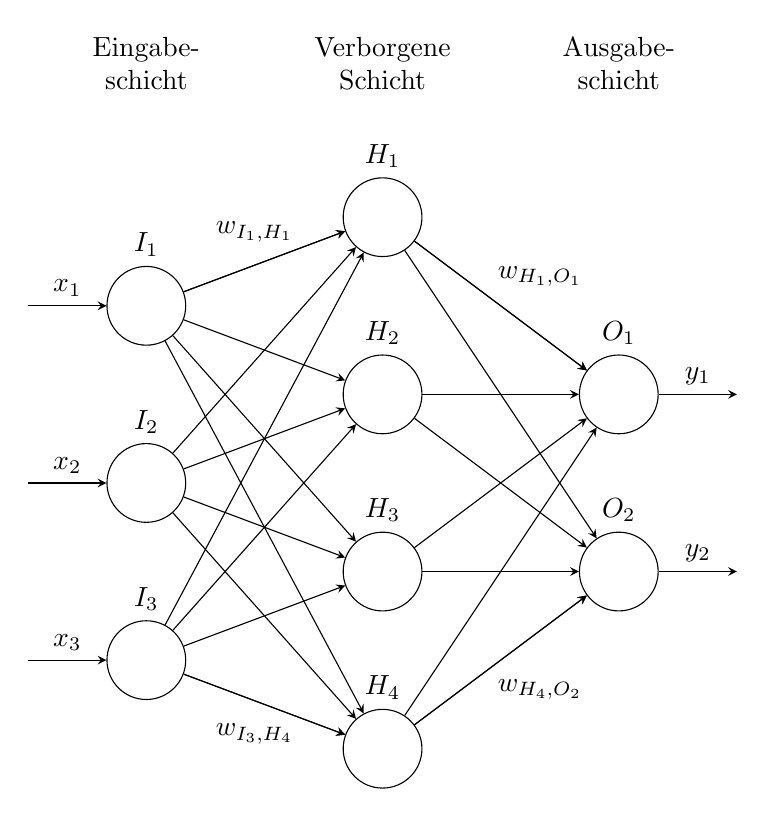
\begin{tikzpicture}[x=1.5cm, y=1.5cm, >=stealth]


% Neuronen
\foreach \m/\l [count=\y] in {1,2,3}
  \node [every neuron/.try, neuron \m/.try] (input-\m) at (0,1.75-\y*1.5) {};

\foreach \m [count=\y] in {1,2,3,4}
  \node [every neuron/.try, neuron \m/.try ] (hidden-\m) at (2,2.5-\y*1.5) {};

\foreach \m [count=\y] in {1,2}
  \node [every neuron/.try, neuron \m/.try ] (output-\m) at (4,1-\y*1.5) {};


% Beschriftungen für Ein- und Ausgänge
\foreach \l [count=\i] in {1,2,3}
	\draw [<-] (input-\i) -- ++(-1,0)
		node [above, midway] {$x_\l$};

\foreach \l [count=\i] in {1,2}
	\draw [->] (output-\i) -- ++(1,0)
		node [above, midway] {$y_\l$};


% Neuronen Beschriftungen
\foreach \l [count=\i] in {1,2,3}
	\node [above] at (input-\i.north) {$I_\l$};

\foreach \l [count=\i] in {1,2,3,4}
	\node [above] at (hidden-\i.north) {$H_\l$};

\foreach \l [count=\i] in {1,2}
	\node [above] at (output-\i.north) {$O_\l$};
   

% Verbindungen
\foreach \l [count=\i] in {1,2,3}
  \foreach \k [count=\j] in {1,2,3,4}
    \draw [->] (input-\l) -- (hidden-\k);

\draw [->] (input-1) -- (hidden-1)
	node [above, midway, xshift=-.125cm, yshift=.125cm] {$w_{I_1,H_1}$};
	
\draw [->] (input-3) -- (hidden-4)
	node [below, midway, xshift=-.125cm, yshift=-.125cm] {$w_{I_3,H_4}$};

\foreach \l [count=\i] in {1,2,3,4}
  \foreach \k [count=\j] in {1,2}
    \draw [->] (hidden-\i) -- (output-\j);

\draw [->] (hidden-1) -- (output-1)
	node [above, midway, yshift=.125cm, xshift=.5cm] {$w_{H_1,O_1}$};
	
\draw [->] (hidden-4) -- (output-2)
	node [below, midway, yshift=-.125cm, xshift=.5cm] {$w_{H_4,O_2}$};


% Schichten Beschriftung
\node [align=center, above] at (0,2) {Eingabe- \\ schicht};
\node [align=center, above] at (2,2) {Verborgene \\ Schicht};
\node [align=center, above] at (4,2) {Ausgabe- \\ schicht};

\end{tikzpicture}